\section{Motivation}
\label{sec:Motivation}

\begin{wrapfigure}{r}{0.41\textwidth}
		\centering
		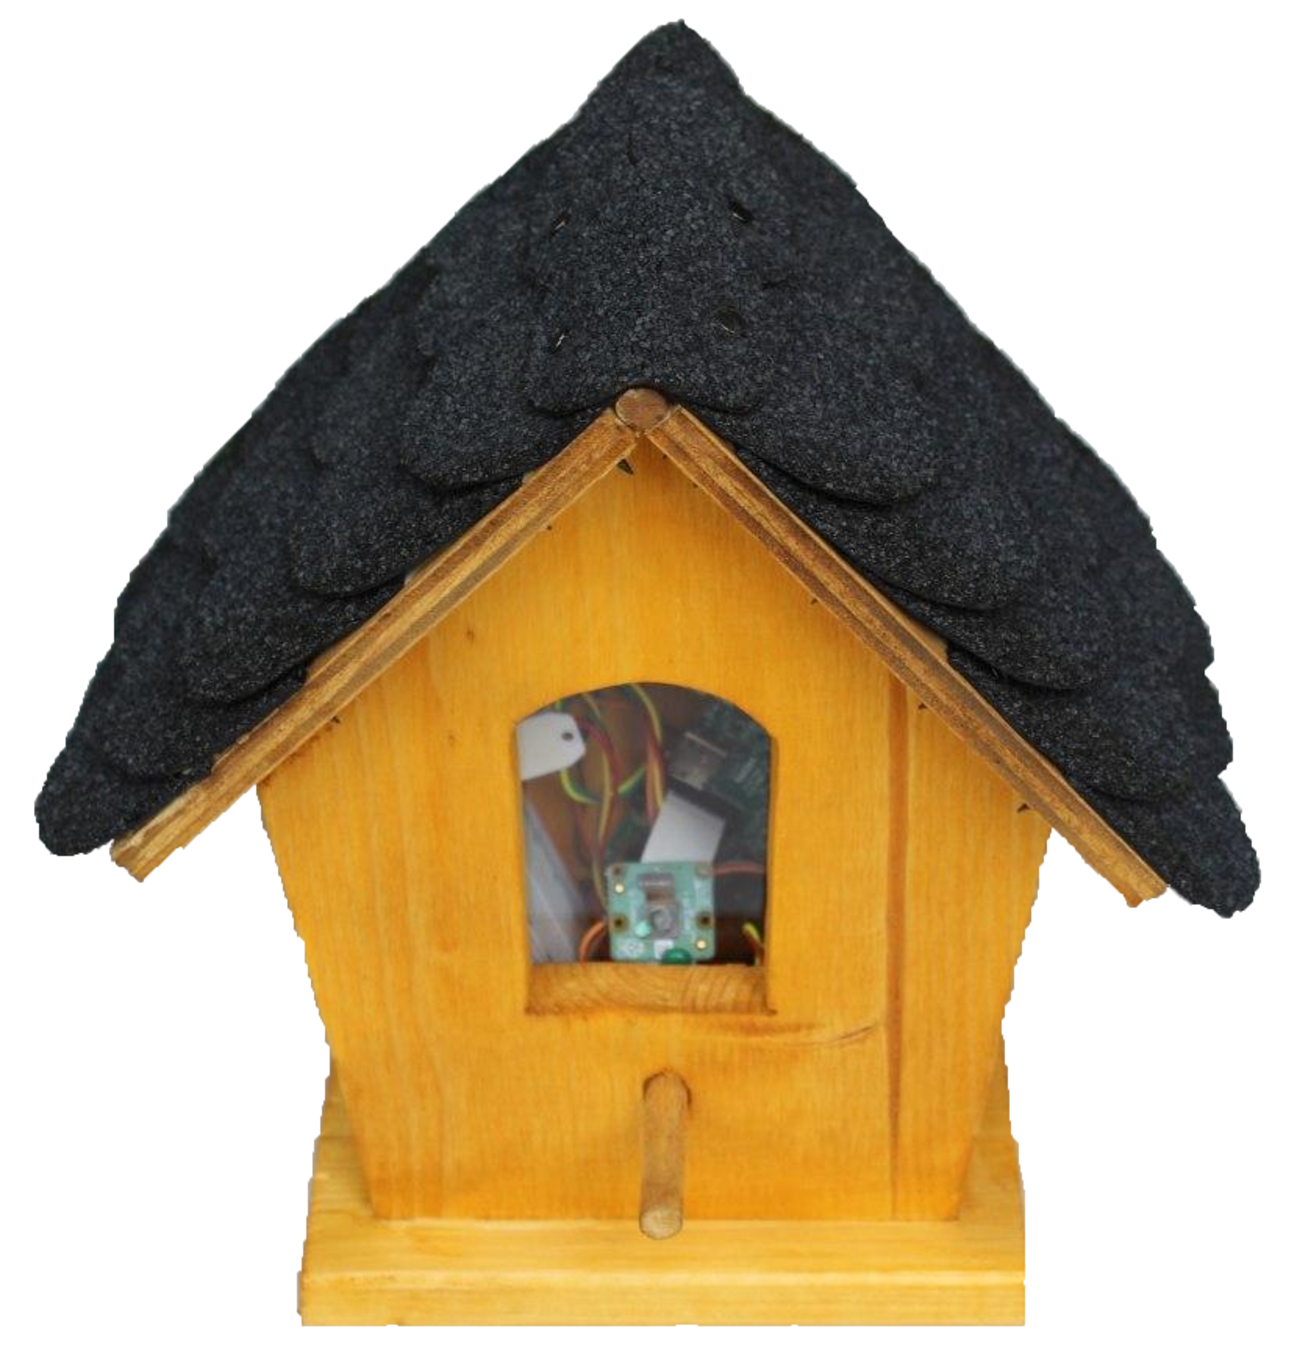
\includegraphics[width=0.4\textwidth]{./pictures/wetterstation.pdf}
		\caption{Wetterstation zur aufnahme der Daten}
		\label{fig:name}
\end{wrapfigure}
Das Weatherpi Projekt entsteht im Rahmen des Physikstudiums.
Es widmet sich der Fragestellung, ob sich mit einfachen Mitteln zuverlässige
Wettervorhersagen erstellen lassen können.
Dazu werden lokale Daten mittels Sensoren welche an einen einfachen Einplatinencomputer
angeschlossen sind, erhoben.
Diese Daten werden anschliessend auf einen Server hochgeladen welcher
flaechendeckende Wettervorhersagen machen soll. \par
Zu den Erhobenen Daten zahlen die Temperatur, der Druck, die Luftfeuchtigkeit
sowie ein Ausschnitt der Wolkendecke.
Um Korrelationen zwischen den Attributen und der Bewoelkung zu entdecken muessen die Daten
bei bekannter Bewoelkung aufgenommen werden.
Zur spezifizierung der aktuellen Wetterlaage ist die Wolkendecke ebenso notwendig.

Die erhobenen Daten sollen mittels einer Live Analyse ausgewertet werden.
Diese steht unter der Permisse schnell, genau und recoursenschonend zu seien.
Dazu werden algorithmen des Maschinellen lernenens verwendet. 
Ziel ist es nach der Erstellung eines klassifizierten Trainingssatzes, die auf
diesem trainierten Algorithmen bei hinreichend grosser genauigkeit die Klassen
automatisiert erkennen zu lassen.
Wenn das Klassenlabel bekannt ist braucht nicht mehr die gesamte Datenmenge des Fotos 
zum Server geschickt werden und der Datentransfer kann reduziert werden. 
Desweiteren kann die Rechenlast auf die RasperryPis welche in der Regel nicht ausgelastet sind, 
vom Server ausgelagert werden. 

Dazu werden zwei Modelle evaluiert welche auf den beiden Charakeristischen
Eigenschaften des Wolkenspektrums trainiert werden. 
Diese sind einerseits die Formen, sowie das Farbspektrum der Wolken.
Aus dem aufgenommenen Foto wird ein diskretes Farbspektrum erstellt, welches mit
einem Random Forest ausgewertet werden kann.
Dabei bietet der Random Forrest ein groesst moeglichen Schutz gegen üebertraining.
Mittels eine Convolutional Neuronal Network (CNN) besteht die Moeglichkeit auf
dem Farbspektrum der Wolken sowie deren Formen zu trainieren. 
Die erhoehte Informationsdichte mit der das CNN trainiert werden kann, verspricht bei 
gutem Training ein einen performance Schub.

Werden die Wolken entsprechend richtig klassifiziert laesst sich in weiteren
Schritten welche nicht Teil dieses Papers sind aus der Folge der Wolken z.B
der Niederschlag berechnen. 
Desweiteren kann die entwicklung der Temperatur aufgrund der Waermespeicherung
und Isolierug von Wolken verbessert werden.

